\documentclass[a4paper, 12pt]{article}
\usepackage[small]{titlesec}
\usepackage[T2A]{fontenc}
\usepackage[utf8]{inputenc}
\usepackage[english,russian]{babel}
\usepackage{graphicx}
\usepackage{amsmath}
\usepackage{listings}
\newcommand\tab[1][1cm]{\hspace*{#1}}
\renewcommand{\baselinestretch}{1.5}

\date{Сентябрь 2020}
\begin{document}
	
	\begin{titlepage}
		\begin{center}
			
\includegraphics{msu_logo.jpg}
			\small
			~\\[0.1cm]
			Московский государственный университет имени М.В.Ломоносова
			~\\[0.1cm]
			Казахстанский филиал
			~\\[0.1cm]
			Факультет вычислительной математики и кибернетики
			~\\[1.0cm]
			\normalsize
		\end{center}
		\vspace{0.5cm}
		\begin{center}
			\textbf{\large{Отчёт по практикуму по специализации}}
			\\[1cm]
			\textbf{\large {Численное решение задачи Дирихле для уравнения
					Пуассона}}
			\\[2cm]
			\begin{normalsize}
				\vspace{2cm}
				\begin{flushright}
					\textbf{Составил}: студент Калдаров Б.М.
					\\[1cm]
					\textbf{Проверил}: преподаватель Нетесов В.В.
				\end{flushright}
				\normalsize
			\end{normalsize}
			\vfill 
			
			\small{Нур-Султан, 2021}
		\end{center} 
	\end{titlepage}
	\setcounter{page}{2}
	\tableofcontents
	
	\newpage
	\section{Постановка задачи}
	Рассматривается задача Дирихле для эллиптического уравнения
	\begin{equation}
		-Lu = f(x, y), \;\;\; (x, y) \in G,
	\end{equation}
	\begin{equation}
		u = \mu(x, y), \;\;\; (x, y) \in H.
	\end{equation}
	Пусть $\overline{G} = G + H = {0 \le x \le l_x, 0 \le y \le l_y}$ - прямоугольник, а
	\begin{equation}
		Lu = \frac{\partial}{\partial x} \bigg( p(x, y) \frac{\partial u}{\partial x} \bigg) + \frac{\partial}{\partial y} \bigg( q(x, y) \frac{\partial u}{\partial y} \bigg)
	\end{equation}
	
	
	Здесь $p(x, y), q(x, y)$ - достаточно гладкие функции такие, что $0 < c_1 \le p(x, y) \le c_2, 0 < d_1 \le q(x, y) \le d_2$, где $c_1, c_2, d_1, d_2$ - постоянные.
	Обозначим $A = max(c_2, d_2)$.
	Разобьём отрезок $[0, l_x]$ на $N_x$ равных частей. Обозначим $h_x = \frac{l_x}{N_x}, x_i = i h_x, 0 \le i \le N_x.$
	\newline
	Разобьём отрезок $[0, l_y]$ на $N_y$ равных частей. Обозначим $h_y = \frac{l_y}{N_y}, y_j = j h_y, 0 \le j \le N_y.$
	\newline
	
	\newpage
	\section{Основные результаты}
	\subsection{Выбор функций и параметров}
	В качестве пробной функции взята функция
	$$\mu(x, y) = x^2 y + y^2 x$$ 
	Правая часть $$ f(x, y) = x y$$
	Норма $|| A || = max | a_{ij} |$, a точность $eps = 1e-2$.
	\newline
	Количество итераций считалось по формулам 
	\newline
	Для метода простой итерации:
	$$ m \ge 2 \frac{ln(1/eps)}{(\pi h)^2}$$	
	Для метода Зейделя:
	$$ m \ge \frac{ln(1/eps)}{(\pi h)^2}$$	
	Для метода верхней релаксации:
	$$ m \ge 2 \frac{ln(1/eps)}{\pi h}$$	
	
	\newpage
	\subsection{Метод простой итерации с оптимальным параметром}
		
	\begin{center}
		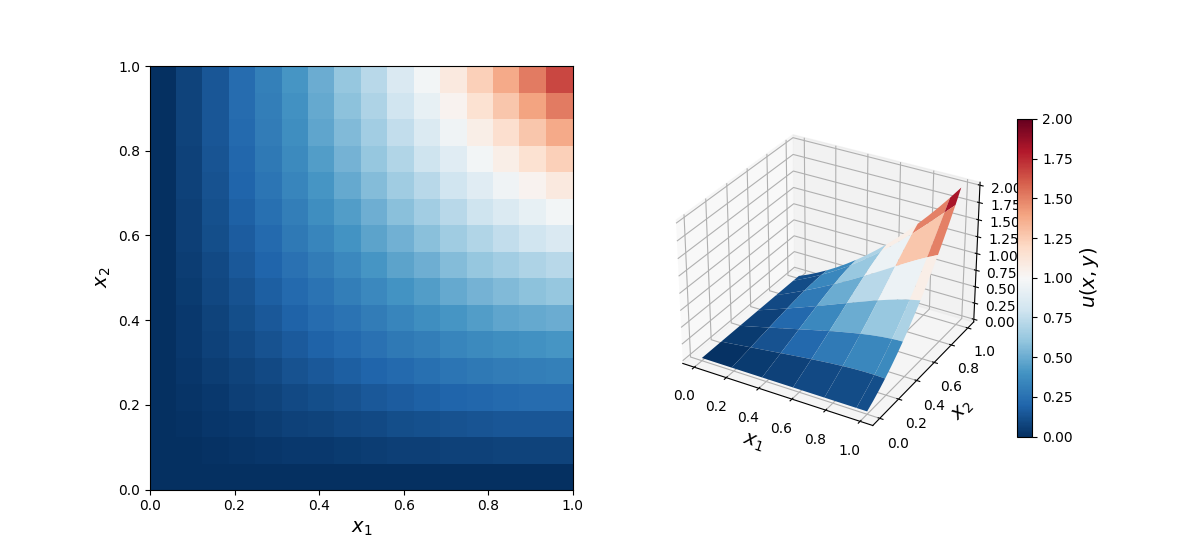
\includegraphics[scale=0.5]{plot11_1.png} \\
		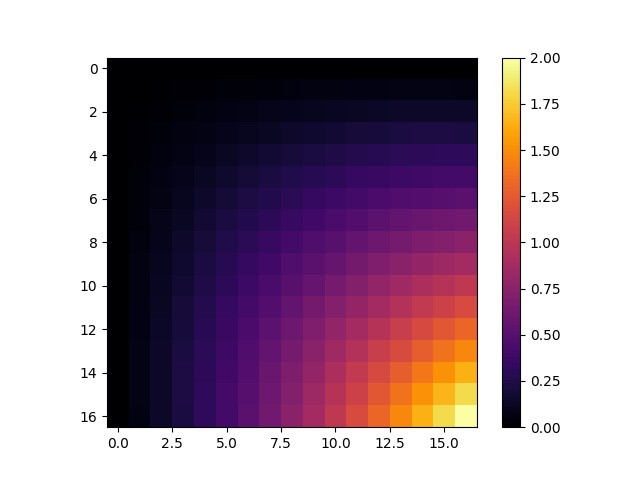
\includegraphics[scale=0.4]{plot11_2.png} \\
		\text{График для } $n = 16, m_{opt} = 239$.
	\end{center}

	\begin{center}
		\begin{tabular}{||c c c c||} 
			\hline
			N & $||u^k-u^*||$ & $\frac{||u^k-u^*||}{||u^0-u^*||}$ & $||u^k-u^{k-1}||$ \\ [0.5ex] 
			\hline\hline
			1 & 1.647 & 0.823 & 2.0 \\ 
			\hline
			10 & 0.712 & 0.356 & 0.0583 \\
			\hline
			30 & 0.26 & 0.13 & 0.013 \\
			\hline
			$m_{opt}$ & 0.025 & 0.0126 & 0.004 \\ [1ex] 
			\hline
		\end{tabular}
	\end{center}

	\newpage
	\subsection{Метод Зейделя}
	
	\begin{center}
		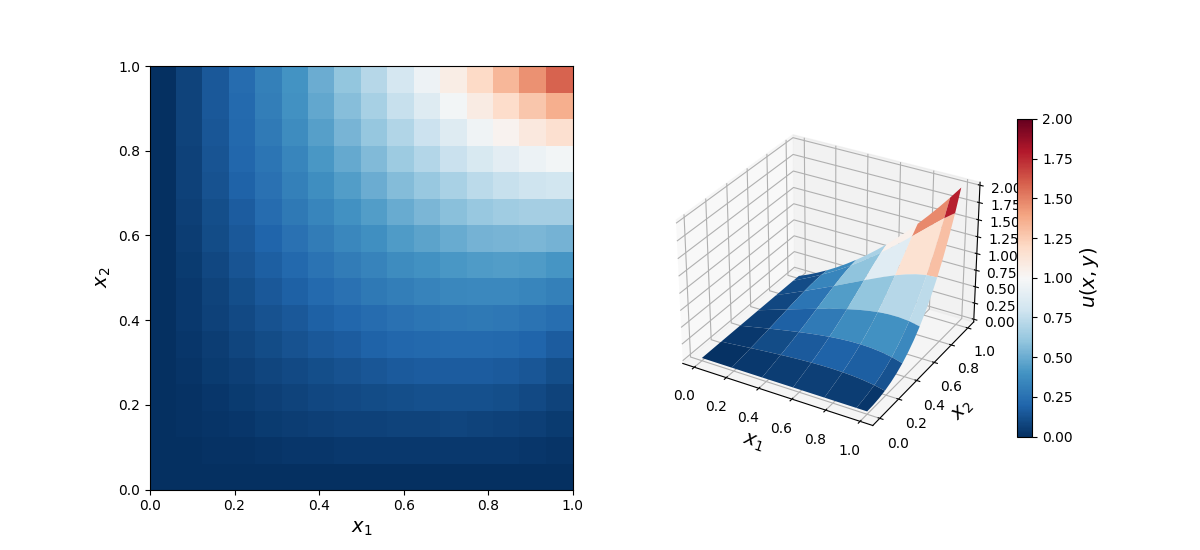
\includegraphics[scale=0.5]{plot22_1.png} \\
		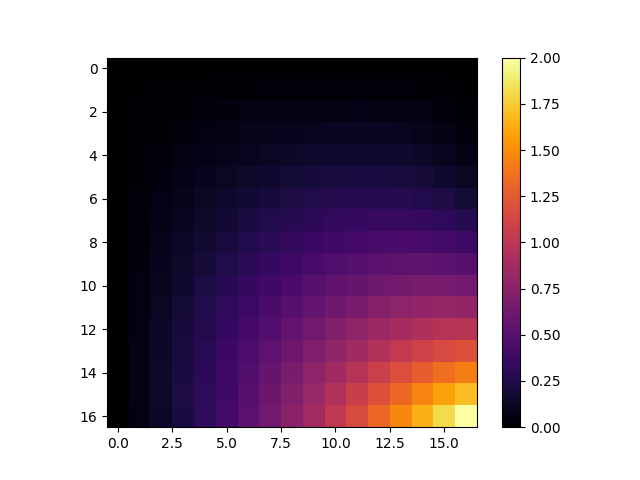
\includegraphics[scale=0.4]{plot22_2.png} \\
		\text{График для } $n = 16, m_{opt} = 120$.
	\end{center}
	
	\begin{center}
		\begin{tabular}{||c c c c||} 
			\hline
			N & $||u^k-u^*||$ & $\frac{||u^k-u^*||}{||u^0-u^*||}$ & $||u^k-u^{k-1}||$ \\ [0.5ex] 
			\hline\hline
			1 & 1.544 & 0.77 & 2.0 \\ 
			\hline
			10 & 0.340 & 0.17 & 0.049 \\
			\hline
			30 & 0.091 & 0.045 & 0.009 \\
			\hline
			$m_{opt}$ & 0.238 & 0.119 & 0.0002 \\ [1ex] 
			\hline
		\end{tabular}
	\end{center}

	\newpage
	\subsection{Метода верхней релаксации}
	
	\begin{center}
		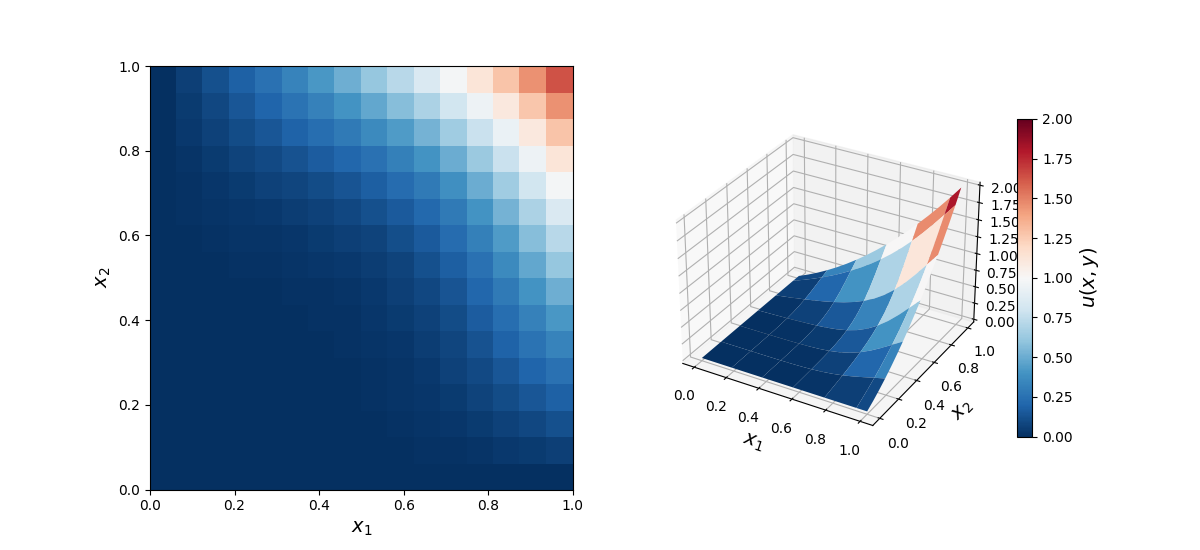
\includegraphics[scale=0.5]{plot33_1.png} \\
		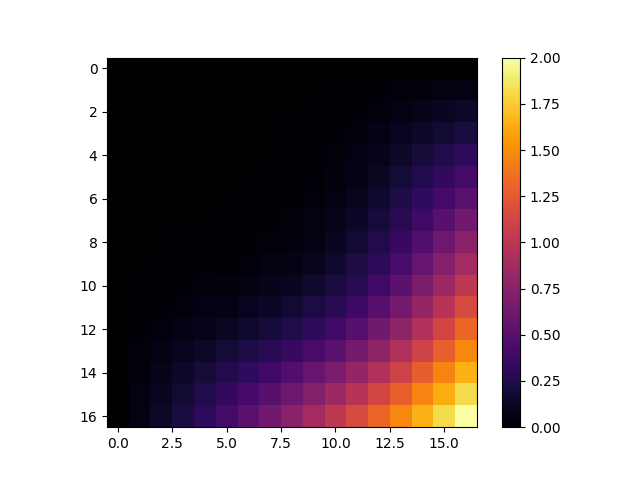
\includegraphics[scale=0.4]{plot33_2.png} \\
		\text{График для } $n = 16, m_{opt} = 47$.
	\end{center}
	
	\begin{center}
		\begin{tabular}{||c c c c||} 
			\hline
			N & $||u^k-u^*||$ & $\frac{||u^k-u^*||}{||u^0-u^*||}$ & $||u^k-u^{k-1}||$ \\ [0.5ex] 
			\hline\hline
			1 & 1.647 & 0.823 & 2.0 \\ 
			\hline
			10 & 0.861 & 0.43 & 0.057 \\
			\hline
			30 & 0.438 & 0.219 & 0.015 \\
			\hline
			$m_{opt}$ & 0.272 & 0.136 & 0.008 \\ [1ex] 
			\hline
		\end{tabular}
	\end{center}


	
	\newpage
	\section{Листинг программы}
	\subsection{Общий код}
	\lstset{language=Python}
	\begin{lstlisting}[
		basicstyle=\small, %or \small or \footnotesize etc.
		]
# -*- coding: utf-8 -*-
"""
Created on Sun Apr  4 17:55:38 2021

@author: Kaldarov
"""

import numpy as np
import time

import matplotlib as mpl
import matplotlib.pyplot as plt
from mpl_toolkits.mplot3d.axes3d import Axes3D

def norm(a):
	return np.max(np.abs(a))

def mu(x, y):
	return x*x*y + x*y*y

def f(x, y):
	return x * y 

N = 16 
N1 = N+1
L = 1.0 
h = L/N
x = np.linspace(0.0, L, N1)
y = np.linspace(0.0, L, N1)

ua = np.zeros((N1,N1))
for i in range(N1):
	for j in range(N1):
		ua[i, j] = mu(x[i], y[j])

u = np.zeros((N1, N1))

u0 = u.copy()
u_old = u.copy()

delta = 8/(h*h) * np.sin(np.pi*h/2)**2
delta2 = 8/(h*h) * np.cos(np.pi*h/2)**2
xi = delta/delta2

roH = (1-xi)/(1+xi)
print('roH = ', roH)

err = norm(u_old-ua)
eps = 1e-2	
\end{lstlisting}

\newpage
	\subsection{Метод простой итерации с оптимальным параметром}
	\lstset{language=Python}
	\begin{lstlisting}[
		basicstyle=\small, %or \small or \footnotesize etc.
		]
m = int(2*(np.log(1/eps))/(np.pi*h)**2+1)
while m > 0:
	for i in range(N1):
		u_old[i, 0] = mu(x[i], 0.0)
		u_old[i, N] = mu(x[i], 1.0)
		u_old[0, i] = mu(0.0, y[i])
		u_old[N, i] = mu(1.0, y[i])
		
	for i in range(1, N):
		for j in range(1, N):
			u[i, j] = (u_old[i-1, j] + u_old[i+1, j] + 
			u_old[i, j-1] + u_old[i, j+1] + 
			h*h*f(x[i], y[j])) / 4
	
	u, u_old = u_old, u
	err = norm(u - ua)
	print(err, err / norm(u0-ua), norm(u_old-u))
	m -= 1
	\end{lstlisting}
\newpage
	\subsection{Метод Зейделя}
	\lstset{language=Python}
	\begin{lstlisting}[
		basicstyle=\small, %or \small or \footnotesize etc.
		]
m = int((np.log(1/eps))/(np.pi*h)**2+1)
while m > 0:
	for i in range(N1):
		u_old[i, 0] = mu(x[i], 0.0)
		u_old[i, N] = mu(x[i], 1.0)
		u_old[0, i] = mu(0.0, y[i])
		u_old[N, i] = mu(1.0, y[i])


	for i in range(1, N):
		for j in range(1, N):
			u[i, j] = (u[i-1, j] + u_old[i+1, j] + 
			u[i, j-1] + u_old[i, j+1] + 
			h*h*f(x[i], y[i])) / 4
	
	u, u_old = u_old, u
	err = norm(u - ua)
	m -= 1
	print(err, err / norm(u0-ua), norm(u_old-u))
	\end{lstlisting}
\newpage
	\subsection{Метода верхней релаксации}
	\lstset{language=Python}
	\begin{lstlisting}[
		basicstyle=\small, %or \small or \footnotesize etc.
	]
m = int(2*(np.log(1/eps))/(np.pi*h)+1)
while m > 0:
	for i in range(N1):
		u_old[i, 0] = mu(x[i], 0.0)
		u_old[i, N] = mu(x[i], 1.0)
		u_old[0, i] = mu(0.0, y[i]) 
		u_old[N, i] = mu(1.0, y[i])
	
	for i in range(1, N):
		for j in range(1, N):
			u[i, j] = u_old[i, j] + w * (u[i-1, j] + 
			u_old[i+1, j] + u[i, j-1] + u_old[i, j+1] + 
			h*h*f(x[i], y[i]) - 4 * u_old[i, j]) / 4 
	
	u, u_old = u_old, u
	err = norm(u - ua)
	m -= 1
	print(err, err / norm(u0-ua), norm(u_old-u))
 	\end{lstlisting}
	\newpage
	\section{Список литературы}
	
	\begin{enumerate}
		\item \textbf{Пакулина А.Н.} Практикум по методам вычислений. Часть 2. СПб., СПбГУ, 2019. – 113 с.
		\item \textbf{Самарский А.А, Гулин А.В.} Численные методы математической физики. Наука, 2000. - 310 с.
	\end{enumerate}
	
	
	
\end{document}
